\documentclass{article}

\usepackage{graphicx}
\usepackage{pdflscape}
\setlength{\parskip}{1em}

\begin{document}

	\title{EMISY project report:\\Thermal-paper-based optical storage medium
	reading device}
	\author{Michał Szopiński\\\\
	https://github.com/Lachcim/szopinski-emisy}
	\date{April 2, 2021}
	\maketitle
	
	\setcounter{section}{-1}
	\section{Abstract}
	
	The goal of this project was to design a device capable of reading binary
	data from a tape of 80-millimeter thermal paper on which information is
	encoded as a series of black and white squares. The device was to
	communicate with the host computer over the Universal Serial Bus, which
	would enable the data to be collected and recorded by a dedicated computer
	program.
	
	Described in this document are the engineering challenges faced during the
	construction of the machine as well as detailed descriptions of their
	solutions. The project was successfully completed using real hardware.
	
	\newpage
	\renewcommand{\baselinestretch}{0}\normalsize
	\tableofcontents
	\renewcommand{\baselinestretch}{1}\normalsize
	
	\newpage
	\section{Introduction}
	
	Among the first storage media ever used in computing were punched cards and
	punched tape. Although simple in concept, these media are difficult to read
	quickly and accurately using analog circuitry alone. Combining the
	straightforwardness of the past with the robustness of the present, a
	simple microcontroller system may be devised to ensure that they are
	processed in a swift and reliable manner.
	
	To simplify and accelerate the production of sample media to be used with
	the device, thermal paper was chosen in place of the punched tape. Owing to
	the ubiquity and simplicity of generic point-of-sale linear thermal
	printers, any modern computer may be used to produce data tapes without the
	need for any additional drivers.
	
	Both reading and writing of the data tapes is achieved using a simple
	command line interface utility named \texttt{thermfile}, which comes
	bundled with the source code for this project. The implementation of said
	program is outside the scope of this document.
	
	\subsection{Description of the data format}
	
	Below is an illustration showing an example data tape with an explanation
	of its characteristic features. As the device pulls the tape through the
	read head, the symbols are scanned from top to bottom.
	
	As seen on figure~\ref{fig:horizontal}, the tape is split into 10
	machine-readable data tracks and an extra human-readable text track. The
	leftmost 8 tracks encode the 8 bits of a byte, with the least significant
	bit towards the right. The text track provides a handy reference as to what
	data is represented by each symbol.
	
	Because the machine has no control over the absolute position of the tape
	and can only approximately control its speed, a synchronization signal must
	be introduced to ensure that the symbols are read correctly. A pattern of
	alternating ones and zeros is printed on the sync track, marking the start
	and end of a symbol.
	
	Finally, the invert track is used to signify that the data bits of a symbol
	are logically inverted, i.e., ones are represented by zeros and vice-versa.
	This is due to a technical limitation of thermal printers whereby an
	excessive burn area causes a voltage drop in the printer's power rail,
	deteriorating the printout quality. The invert track ensures that at most
	50\% of horizontal space is only ever utilized.
	
	\begin{landscape}
		\begin{figure}[h]
			\minipage{0.5\textwidth}
				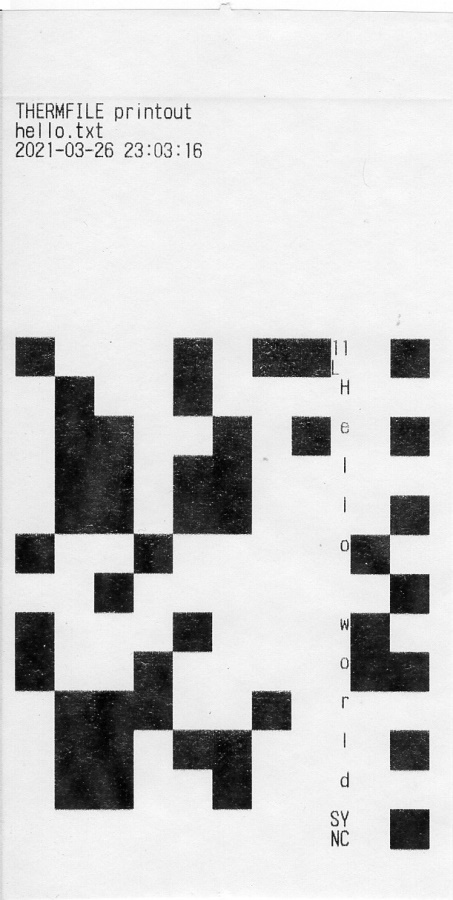
\includegraphics[width=\linewidth]{img/helloworld}
				\caption{Sample data tape}
			\endminipage\hfill
			\minipage{0.5\textwidth}
				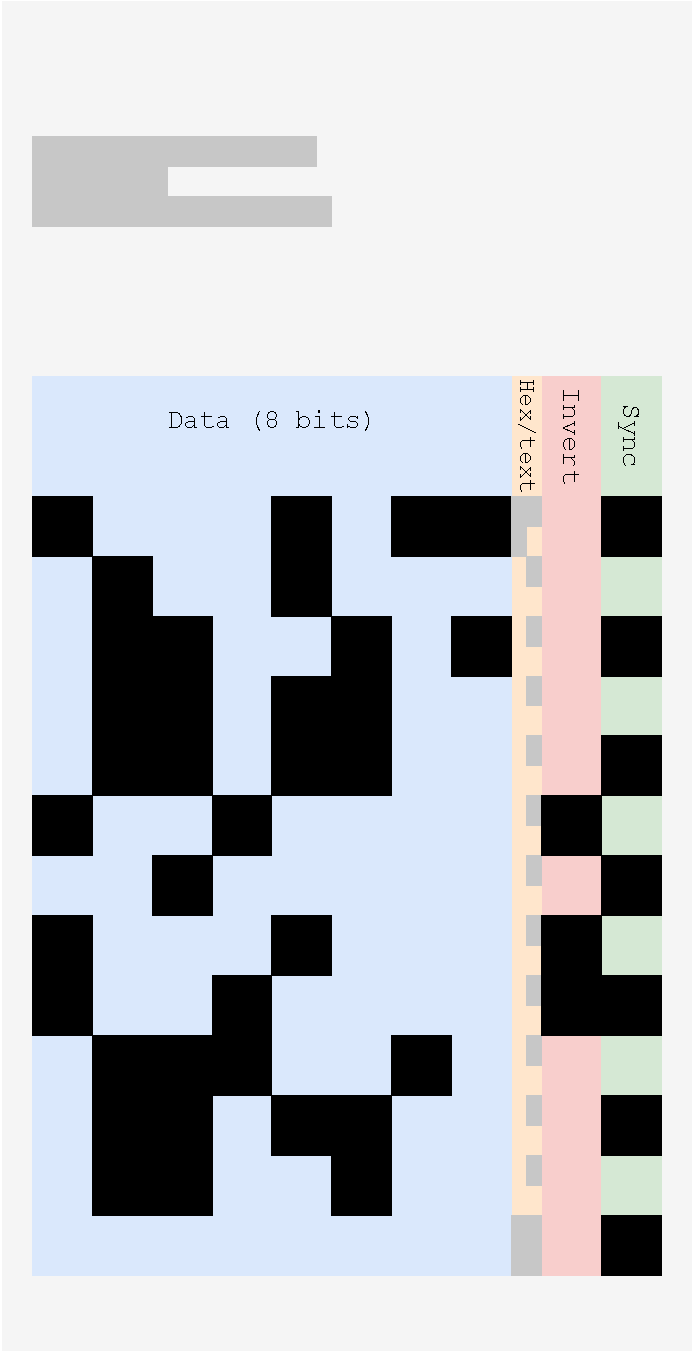
\includegraphics[width=\linewidth]{img/horizontal}
				\caption{Horizontal layout}
				\label{fig:horizontal}
			\endminipage\hfill
			\minipage{0.5\textwidth}
				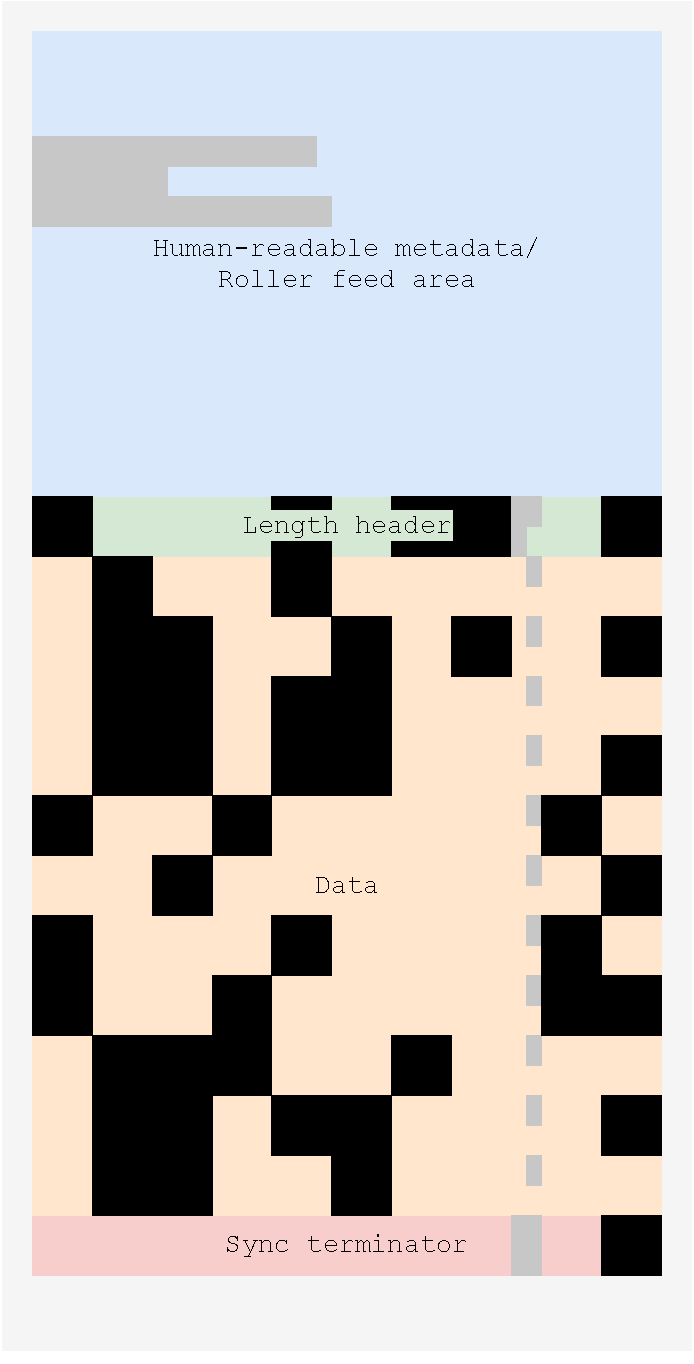
\includegraphics[width=\linewidth]{img/vertical}
				\caption{Vertical layout}
				\label{fig:vertical}
			\endminipage
		\end{figure}
	\end{landscape}
	
	Figure~\ref{fig:vertical} shows the vertical layout of symbols on the tape.
	Each printout begins with a large blank area on which human-readable
	metadata is printed for convenience. This area allows the user to push the
	tape through the read head chamber to be taken up by the roller.
	It also participates in the two-step read initialization process discussed
	in section~\ref{sec:software}.
	
	As a simple error detection measure, the device is informed about the
	length of the incoming data in advance. This information is carried by the
	length header, present at the start of the data track. Each line of the
	header carries 7 bits of the length value, in little endian order. The
	most significant bit marks the end of the length header.
	
	Past the header, binary data begins. The start and end positions of a
	symbol are determined by detecting a change in the synchronization signal.
	If there is an odd number of symbols on the tape, the final sync signal is
	white and therefore indistinguishable from the white margin of the tape.
	For this reason, a sync terminator is introduced to mark the end of
	odd-numbered final symbols.
	
	\subsection{Communication protocol}
	
	Having no hardware resources required for independent operation, the device
	is granted very little autonomy in terms of its work cycle. The only
	physical control present on its body is the emergency stop button --
	otherwise, session initialization, session halting, and data collection are
	all governed by the host computer.
	
	A simple communication protocol is used to exchange data and status
	messages with the \texttt{thermfile} utility running on the computer. Each
	packet begins with a single byte identifying the type of the message and a
	fixed-size payload. The messages enter and leave the microcontroller
	through UART. USB communication is handled by specialized hardware and
	software.
	
	\subsubsection{Table of messages}
	
	\begin{center}
		\begin{tabular}{ |c|c|p{7cm}|c| }
		\hline
			Code & Direction & Meaning & Payload \\
		\hline
			\texttt{S} &
			To device &
			\textbf{Start read}\newline
			Enables power to the read head and starts the roller motor. Begins
			the read session.
			& 0 \\
		\hline
			\texttt{C} &
			To host &
			\textbf{Start read confirm}\newline
			Confirms the start read instruction.
			& 0 \\
		\hline
			\texttt{L} &
			To host &
			\textbf{Incoming data length}\newline
			Announces the length of the incoming data. The payload is a 64-bit
			little-endian value describing the length.
			& 8 \\
		\hline
			\texttt{D} &
			To host &
			\textbf{Incoming data}\newline
			Marks a single byte of the incoming data.
			& 1 \\
		\hline
			\texttt{F} &
			To host &
			\textbf{Read finished}\newline
			Sent once the read session is finished and a new session may be
			initialized.
			& 0 \\
		\hline
			\texttt{E} &
			To host &
			\textbf{Error}\newline
			Signals an error which caused the read session to abort. See the
			table of error codes below.
			& 1 \\
		\hline
			\texttt{X} &
			To device &
			\textbf{Emergency stop}\newline
			Triggers an emergency stop error and halts the read session. The
			device responds with an error code.
			& 0 \\
		\hline
		\end{tabular}
	\end{center}
	
	\subsubsection{Table of error codes}
	
	\begin{center}
	\begin{tabular}{ |c|p{9cm}| }
		\hline
			Error code & Meaning \\
		\hline
			\texttt{I} &
			\textbf{Initialization timeout}\newline
			The first symbol failed to appear within the set timeframe. \\
		\hline
			\texttt{R} &
			\textbf{Read timeout}\newline
			The next symbol failed to appear within the set timeframe. \\
		\hline
			\texttt{E} &
			\textbf{Emergency stop}\newline
			An emergency stop was triggered either by the stop button or
			remotely. \\
		\hline
			\texttt{B} &
			\textbf{Serial buffer busy}\newline
			An attempt to send data was made before the serial buffer had been
			cleared. This error is indicative of a too high scan rate and does
			not occur under ordinary working conditions.\\
		\hline
		\end{tabular}
	\end{center}
	
\end{document}
